
\section{Case study: Oral carcinomas vs matched normal tissue}\label{tuch}
\subsection{Introduction}
This section provides a detailed analysis of data from a paired design
RNA-seq experiment, featuring oral squamous cell carcinomas and
matched normal tissue from three patients \citep{Tuch:2010p457}. For a
paired design, as we discussed before, we have to apply the Cox-Reid
(CR) method in estimating dispersions and the GLM method in detecting
DE tags.

\subsection{Source of the data}
The dataset is obtained from the NCBI's Gene Expression Omnibus (GEO)
(\url{http://www.ncbi.nlm.nih.gov/geo/}). It was produced using the
Applied Biosystems (AB) SOLiD System 3.0, and is described in
\citet{Tuch:2010p457}. The data downloaded from GEO consisted of a
file for each of the six samples, each of which contained mapped reads
in AB's MAX format (similar to FASTA). The raw reads had been mapped
by \citet{Tuch:2010p457} to the UCSC hg18 reference genome. In order
to analyse these data in \R\ it was necessary to generate, from the
MAX files, a file for each sample that contained the number of counts
for each gene sequenced and successfully mapped, as well as the gene
ID's corresponding to the reads.

AB supply some software tools for the analysis of RNA-seq data from
the SOLiD platform. One function, \code{count\_tags.pl} exists to
count the number of reads mapping to each position of the genome and
provide the associated gene and transcript ID's, as well as other
information such as chromosome and precise start and end points of the
read.

According to \citet{Tuch:2010p457}'s paper, the reads were mapped to
the UCSC hg18 reference genome. A reference annotation file was
created using the AB function \code{refgene2gff.sh} (the default
annotation for the AB software).

The file produced by \code{count\_tags.pl} contains a row for each
unique exon position in the genome to which reads map. For each row
there are many columns which provide information including the
matching gene and transcript ID's, the starting point and ending
points for the reads and the count (number) of reads for that position
in the genome. One such file was produced for each of the six samples.

The final task to produce data files that \edgeR\ can handle was to
simplify the files output by \code{count\_tags.pl} into files with
just one row for each gene ID and the appropriate count for each gene
ID.

\subsection{Reading in the data and creating a \texttt{DGEList} object}

Our first task is to load the \edgeR\ package, read the data into \R\
and organise the data into a \texttt{DGEList} object that the
functions in the package can recognise. The library size is usually
the total sum of all of the counts for a library, and that is how
library size is defined in this analysis. The easiest way to construct
an appropriate \texttt{DGEList} object for these data is described
below. In this case, the tag counts for the four individual libraries
are stored in six separate plain text files.

In each file, the tag IDs and counts for each tag are provided in a
table. It is best to create a tab-delimited, plain-text `Targets'
file, which, under the headings `files', `group' and `description',
gives the filename, the experimental group and a brief description for
each sample.

The \texttt{targets} object is produced when the \texttt{Targets.txt}
file is read into the \R\ session. This object makes a convenient
argument to the function \texttt{readDGE} which reads the tables of
counts into our \R\ session, calculates the sizes of the count
libraries and produces a \texttt{DGEList} object for use by subsequent
functions.


\begin{Schunk}
\begin{Sinput}
> library(edgeR)
> setwd("/Users/dmccarthy/Documents/DGE/TuchData")
> targets <- read.delim(file = "targets.txt", stringsAsFactors = FALSE)
> targets$tissue <- factor(targets$group)
> targets$patient <- factor(c(8, 8, 33, 33, 51, 51))
> targets
\end{Sinput}
\begin{Soutput}
                              files  group
1  GSM515513_N8_gene_agg_counts.txt normal
2  GSM515514_T8_gene_agg_counts.txt tumour
3 GSM515515_N33_gene_agg_counts.txt normal
4 GSM515516_T33_gene_agg_counts.txt tumour
5 GSM515517_N51_gene_agg_counts.txt normal
6 GSM515518_T51_gene_agg_counts.txt tumour
                                          description tissue patient
1                 healthy mouth tissue from patient 8 normal       8
2  oral squamous cell carcinoma tissue from patient 8 tumour       8
3                healthy mouth tissue from patient 33 normal      33
4 oral squamous cell carcinoma tissue from patient 33 tumour      33
5                healthy mouth tissue from patient 51 normal      51
6 oral squamous cell carcinoma tissue from patient 51 tumour      51
\end{Soutput}
\begin{Sinput}
> d.tuch <- readDGE(targets, skip = 1, comment.char = "#")
> colnames(d.tuch) <- c("N8", "T8", "N33", "T33", "N51", "T51")
> d.tuch <- calcNormFactors(d.tuch)
> d.tuch
\end{Sinput}
\begin{Soutput}
An object of class "DGEList"
$samples
                                files  group
N8   GSM515513_N8_gene_agg_counts.txt normal
T8   GSM515514_T8_gene_agg_counts.txt tumour
N33 GSM515515_N33_gene_agg_counts.txt normal
T33 GSM515516_T33_gene_agg_counts.txt tumour
N51 GSM515517_N51_gene_agg_counts.txt normal
T51 GSM515518_T51_gene_agg_counts.txt tumour
                                            description tissue patient lib.size
N8                  healthy mouth tissue from patient 8 normal       8  8859892
T8   oral squamous cell carcinoma tissue from patient 8 tumour       8  8270556
N33                healthy mouth tissue from patient 33 normal      33 17635449
T33 oral squamous cell carcinoma tissue from patient 33 tumour      33 15741712
N51                healthy mouth tissue from patient 51 normal      51 24009496
T51 oral squamous cell carcinoma tissue from patient 51 tumour      51 16967249
    norm.factors
N8     1.1510827
T8     1.0695499
N33    0.7049137
T33    0.9524320
N51    1.0427154
T51    1.1602638

$counts
         N8  T8   N33  T33   N51  T51
A1CF      0   0     0    0     0    0
A2BP1   188   1   154    1   711   57
A2LD1    10   0    18   13    40   22
A2M    2238 261  2375  612 15351 2003
A2ML1 11751 911 13305 3080  6935 1156
21783 more rows ...
\end{Soutput}
\end{Schunk}

This \texttt{DGEList} is now ready to be passed to the functions that
do the calculations to determine differential expression levels for
the genes. Note that when we `see' the \texttt{DGEList} object
\texttt{d.tuch}, the counts for just the first five genes in the table
are shown, as well as the \texttt{samples} element, which is a data
frame constructed from the `Targets.txt' file and provides the
filenames, groups, descriptions and library sizes for the samples.

However, for this dataset, there were over 20 000 unique tags
sequenced, some of which have a very small number of counts in total
across all libraries. It is not possible to achieve statistical
significance with fewer than ten counts in total for a tag, and we
also do not want to waste effort finding spurious DE (such as when a
gene is only expressed in one library), so we filter
out tags with fewer than 1 count per million in four or more libraries---this
also helps to speed up the calculations we need to perform. The
subsetting capability of \texttt{DGEList} objects makes such filtering
very easy to carry out.

\begin{Schunk}
\begin{Sinput}
> d.tuch <- d.tuch[rowSums(1e+06 * d.tuch$counts/expandAsMatrix(d.tuch$samples$lib.size, 
+     dim(d.tuch)) > 1) >= 2, ]
> nrow(d.tuch)
\end{Sinput}
\begin{Soutput}
[1] 15318
\end{Soutput}
\end{Schunk}

Now the dataset is ready to be analysed for differential expression.

\subsection{Producing an MDS plot}

Before proceeding with the computations for differential expression,
it is possible to produce a plot showing the sample relations based on
multidimensional scaling. The function \texttt{plotMDS.dge} produces
an MDS plot for the samples when provided with the \texttt{DGEList}
object, as shown in Figure~\ref{fig:Tuch_MDS}.

\begin{Schunk}
\begin{Sinput}
> png(file = "edgeR_case_study_Tuch_MDSplot.png", height = 600, 
+     width = 600)
> plotMDS.dge(d.tuch, main = "MDS Plot for Tuch Data")
\end{Sinput}
\begin{Soutput}
Using grid search to estimate tagwise dispersion. 
\end{Soutput}
\begin{Sinput}
> dev.off()
\end{Sinput}
\begin{Soutput}
null device 
          1 
\end{Soutput}
\end{Schunk}

From the MDS plot, it can be seen that the libraries T33 and T8
(tumour samples from patients 33 and 8 respectively) are most
different from the other samples, but we will not remove them from the
analysis as we will just be demonstrating the use of \edgeR.

\begin{figure}[ht]
\begin{center}
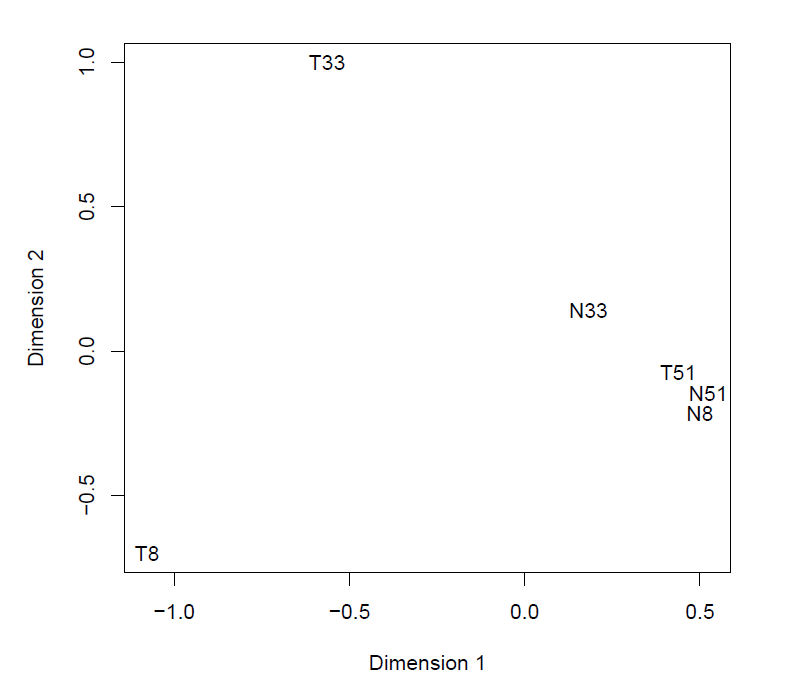
\includegraphics[height=0.45\textheight]{edgeR_case_study_Tuch_MDSplot.png}
\caption{Multidimensional scaling (MDS) plot for the Tuch data,
  showing the relations between the samples in two dimensions. From
  this plot, the samples T33 and T8 can be identified easily as outliers---there is a large distance between these two samples and the others.}
\label{fig:Tuch_MDS}
\end{center}
\end{figure}

\subsection{The design matrix}

Before we fit negative binomial GLMs, we need to define our design
matrix based on the experimental design. Here we want to test for
differential expressions between tumour and normal tissues within
patients, i.e.~adjusting for differences between patients. In
statistical terms, this is an additive linear model with patient as
the blocking factor. So the full design matrix can be created as
follows.

\begin{Schunk}
\begin{Sinput}
> design <- model.matrix(~patient + tissue, data = targets)
> design
\end{Sinput}
\begin{Soutput}
  (Intercept) patient33 patient51 tissuetumour
1           1         0         0            0
2           1         0         0            1
3           1         1         0            0
4           1         1         0            1
5           1         0         1            0
6           1         0         1            1
attr(,"assign")
[1] 0 1 1 2
attr(,"contrasts")
attr(,"contrasts")$patient
[1] "contr.treatment"

attr(,"contrasts")$tissue
[1] "contr.treatment"
\end{Soutput}
\end{Schunk}

This is the design matrix under the alternative hypothesis (i.e.~the
difference between the normal tissue and the tumour tissue does
exist), and the design matrix under the null hypothesis is just the
above matrix without the last column.


\subsection{Analysis using Cox-Reid common dispersion}

\subsubsection{Estimating the Cox-Reid common dispersion}

The first major step in the analysis of DGE data using the NB model is
to estimate the dispersion parameter for each tag. Note that this is a
paired design experiment, so the dispersion has to be estimated in a
different way such that both the cell-type and the patient factors are
taken into account.

Like the qCML method (i.e.,the \texttt{estimateCommonDisp()} and the
\texttt{estimateTagwiseDisp()} function) we used in previous case
studies, the CR method also calculates both the common dispersion and
tagwise dispersions. The most straight-forward analysis for a paired
design experiment uses the CR common dispersion estimate as the
dispersion for all tags. For many applications this will be adequate
and it may not be necessary to estimate the CR tagwise dispersions,
i.e.~estimate the CR dispersion separately for each tag.

Estimating the CR common dispersion is done using the function
\texttt{estimateGLMCommonDisp()}. Once we have the design matrix, we
pass it to the \texttt{estimateGLMCommonDisp()} function, together
with the \texttt{DGEList} object `d.tuch'.
\begin{Schunk}
\begin{Sinput}
> d.tuch <- estimateGLMCommonDisp(d.tuch, design)
> names(d.tuch)
\end{Sinput}
\begin{Soutput}
[1] "samples"           "counts"            "common.dispersion"
\end{Soutput}
\end{Schunk}

The output of \code{estimateCRDisp} is a \texttt{DGEList} object with
several new elements. The element \texttt{common.dispersion}, as the
name suggests, provides the estimate of the Cox-Reid common
dispersion, and \texttt{design} gives the design matrix as we defined at
the start.

Under the negative binomial model, the square root of the common
dispersion gives the coefficient of variation of biological
variation. Here the common dispersion is found to be



\begin{Schunk}
\begin{Sinput}
> d.tuch$common.dispersion
\end{Sinput}
\begin{Soutput}
[1] 0.209996
\end{Soutput}
\begin{Sinput}
> sqrt(d.tuch$common.dispersion)
\end{Sinput}
\begin{Soutput}
[1] 0.4582532
\end{Soutput}
\end{Schunk}

\subsubsection{Testing}
Once we have an estimate of the CR common dispersion, we can proceed
with testing procedures for determining differential expression. Since
this is a paired design experiment, we have to use the new testing
method, the GLM method, rather than the exact test (the one we
demonstrated in the previous case studies).

The GLM method fits a negative binomial generalized linear model for
each gene/tag with the unadjusted counts provided, a value for the
dispersion parameter and, optionally, offsets and weights for
different libraries or transcripts. This is done using the funtion
\texttt{glmFit()} and \texttt{glmLRT()}.

The function \texttt{glmFit()} calls the in-built function
\texttt{glm.fit()} to fit the NB GLM for each tag and produces an
object of class \texttt{DGEGLM}. Once we have a fit for a given design
matrix, \texttt{glmLRT()} can be run with a given coefficient or
contrast specified and evidence for differential expression can be
assessed using a likelihood ratio test. The \texttt{glmLRT} function
produces an object of class \texttt{DGELRT} with a table containing
the abundance of each tag (log-concentration, logConc), the log-fold
change of expression between conditions/contrasts being tested
(logFC), the likelihood ratio statistic (LR.statistic) and the p-value
from the LR test (p.value), for each tag in the dataset. Then tags can
be ranked in order of evidence for differential expression, based on
either the $p$-value or the log-fold change of expression computed for
each tag.

The results of the NB GLM likelihood ratio test can be accessed
conveniently using the \texttt{topTags} function applied to the object
produced by \texttt{glmLRT}. The user can specify the number,
\texttt{n}, of tags for which they would like to see the differential
expression information, ranked by $p$-value (default) or fold
change. As the same test is conducted for many thousands of tags,
adjusting the $p$-values for multiple testing is recommended. The
desired adjustment method can be supplied by the user, with the
default method being Benjamini and Hochberg's approach for controlling
the false discovery rate (FDR)~\citep{Benjamini95}. The table below
shows the top $10$ DE genes ranked by $p$-value.

\begin{Schunk}
\begin{Sinput}
> glmfit.tuch <- glmFit(d.tuch, design, dispersion = d.tuch$common.dispersion)
> lrt.tuch <- glmLRT(d.tuch, glmfit.tuch)
> options(digits = 4)
> topTags(lrt.tuch)
\end{Sinput}
\begin{Soutput}
Coefficient: tissuetumour 
          logConc  logFC    PValue       FDR
TMPRSS11B  -8.654 -7.351 5.074e-22 7.773e-18
CKM        -8.083 -7.161 4.690e-20 3.592e-16
TNNC2     -10.123 -6.794 1.047e-19 5.344e-16
MAL        -9.089 -6.852 1.688e-19 6.384e-16
CRNN       -7.129 -7.241 2.084e-19 6.384e-16
PI16      -10.817 -6.547 1.719e-18 4.390e-15
MYBPC1     -8.293 -7.018 2.798e-18 6.123e-15
IL1F6     -10.217 -6.129 7.368e-18 1.411e-14
KRT36     -11.217 -7.356 2.087e-17 3.552e-14
MUC21      -8.938 -6.770 4.265e-17 6.533e-14
\end{Soutput}
\end{Schunk}

The output shows that the \edgeR~package identifies a good deal of
differential expression between the normal tissue group and the tumour
tissue group. The top DE tags are given very small $p$-values, even
after adjusting for multiple testing. Furthermore, all of the top tags
have a large fold change, indicating that these tags are more likely
to be biologically meaningful.

The table below shows the raw counts for the tags that \edgeR~has
identified as the most differentially expressed. For these tags there
seems to be very large differences between the groups, suggesting that
the DE tags identified are truly differentially expressed, and not
false positives.

\begin{Schunk}
\begin{Sinput}
> top <- rownames(topTags(lrt.tuch)$table)
> d.tuch$counts[top, order(d.tuch$samples$group)]
\end{Sinput}
\begin{Soutput}
             N8   N33   N51 T8  T33  T51
TMPRSS11B  2601  7874  3399  3  322    9
CKM        4120  5203 24175  5   24 1225
TNNC2       590  1627  1239  1    8   39
MAL        2742  3977  1772  3  264    8
CRNN      24178 22055 12533 49 2353   26
PI16        231   216  1950  0    2   35
MYBPC1     4791  4145 15766 10   14 1319
IL1F6       367  1825   809 10   45    1
KRT36       711   104    70  2    1    1
MUC21      4161  3432  1722  7  517    5
\end{Soutput}
\end{Schunk}

Note that the 2nd tag ('CKM') and the 7th tag ('MYBPC1') have much
larger counts in patient 55 than in the other two patients, which
shows that the effect from the patients does exist and the GLM method
can pick that up.

If we order the genes by fold change instead of $p$-value, as in the
table below, we see that the tags with the largest fold changes have
very small concentrations. This ranking is dominated by genes that
have zero counts in one group and is less informative than ranking by
$p$-value.

\begin{Schunk}
\begin{Sinput}
> topTags(lrt.tuch, sort.by = "logFC")
\end{Sinput}
\begin{Soutput}
Coefficient: tissuetumour 
         logConc   logFC    PValue       FDR
FBP2      -13.54 -10.089 1.743e-12 2.871e-10
EMX1      -13.42   9.681 2.170e-10 1.741e-08
ATP6V0D2  -13.90   9.653 2.278e-10 1.817e-08
TUSC5     -14.12  -9.436 1.242e-09 7.927e-08
UTS2R     -14.19  -9.419 2.976e-09 1.740e-07
HTR3A     -14.26  -9.242 1.800e-09 1.091e-07
C3orf43   -14.38  -9.143 7.732e-09 4.052e-07
FAM180B   -14.47  -8.967 1.971e-08 9.178e-07
PCSK2     -14.55  -8.869 1.006e-07 3.825e-06
SLCO1B3   -12.74   8.127 9.867e-11 8.588e-09
\end{Soutput}
\begin{Sinput}
> top <- rownames(topTags(lrt.tuch, sort.by = "logFC")$table)
> d.tuch$counts[top, order(d.tuch$samples$group)]
\end{Sinput}
\begin{Soutput}
         N8 N33 N51 T8 T33 T51
FBP2     40  38  28  0   0   0
EMX1      0   0   0 43  67   0
ATP6V0D2  0   0   0 10  55  14
TUSC5    16   8  52  0   0   0
UTS2R     3  22  46  0   0   0
HTR3A    12  20  27  0   0   0
C3orf43  11  21  18  0   0   0
FAM180B  11  10  29  0   0   0
PCSK2    11  21   7  0   0   0
SLCO1B3   1   0   0  2  22 300
\end{Soutput}
\end{Schunk}


We see in the output below that over $2000$ tags are significantly
differentially expressed according to \edgeR~when using the CR common
dispersion estimate and GLM likelihood ratio test. Of those tags,
$491$ are up-regulated in the tumour tissues compared with the normal
tissues and $1691$ are down-regulated in the tumour tissues compared
with normal tissues.

\begin{Schunk}
\begin{Sinput}
> summary(decideTestsDGE(lrt.tuch))
\end{Sinput}
\begin{Soutput}
   [,1] 
-1  1691
0  13136
1    491
\end{Soutput}
\end{Schunk}


\subsection{Cox-Reid dispersions with mean-dependent trend}
\label{sec:cox-reid-dispersions}

It has been noted that the dispersion parameter in RNA-seq data can
depend on the expression level of the gene \citep{Anders:2010p792}. The
function \texttt{estimateGLMTrendedDisp} in \edgeR~estimates
dispersion values that depend on the overall expression level of the
genes. Typically, lowly expressed genes have a higher value for the
dispersion parameter than more highly expressed genes. There are a
number of possible options for the type of trend that is to be fit for
the dispersion parameters. These options are detailed in the help file
for \texttt{estimateGLMTrendedDisp}.

\begin{Schunk}
\begin{Sinput}
> d.tuch <- estimateGLMTrendedDisp(d.tuch, design)
> summary(d.tuch$trended.dispersion)
\end{Sinput}
\begin{Soutput}
   Min. 1st Qu.  Median    Mean 3rd Qu.    Max. 
  0.123   0.147   0.176   0.238   0.277   1.170 
\end{Soutput}
\end{Schunk}

An analysis could be carried out just as for the common dispersion
above, but is not shown here.


\subsection{Analysis using Cox-Reid tagwise dispersion}


\subsubsection{Estimating the Cox-Reid tagwise dispersion}

An extension to simply using the CR common dispersion for each tag is
to estimate the CR dispersion separately for each tag, while
`squeezing' these estimates towards the CR common dispersion estimate
in order to improve inference by sharing information between
tags. This type of analysis can also be carried out in few steps using
the \edgeR~package.

As noted earlier, the dispersion parameter is the overdispersion
relative to the Poisson, and represents the biological, or
sample-to-sample variability. The methods we have developed moderate
the dispersion estimates towards a common dispersion, much like how
the \limma~package moderates the variances in the analysis of
microarray data.

The amount of moderation done is determined by the value of a weight
parameter \code{prior.n}. The value for \code{prior.n} corresponds to
the number of individual tags equivalent to the weight given to the
common likelihood. Thus, the higher \code{prior.n}, the more strongly
the individual dispersion estimates are moderated, or `squeezed',
towards the common value. To run the moderated analysis, we need to
determine how much moderation is necessary. How best to do this is
still an open research question, but we currently recommend selecting
a value for the weight parameter \code{prior.n} \emph{a priori} and
have found that very good results can be obtained this way.

In an experiment such as that we consider here, in which we have just
six samples, with two groups (group factor) and three patients
(blocking factor), and thus two degrees of freedom for estimating the
dispersion parameter. Standard tagwise dispersion estimates are likely
to be unreliable, so we want to give a reasonable weight to the common
likelihood. We need to choose a value for \code{prior.n} such that
individual tagwise dispersion estimates are `squeezed' quite strongly
towards the common dispersion. Here, we choose a moderate amount of
smoothing---we let \code{prior.n} be $8$. This means that the common
likelihood receives the weight of $8$ individual tags, so there will
be a reasonable degree of `squeezing', but there is still ample scope
to estimate an individual dispersion for each tag.

The function \code{estimateGLMTagwiseDisp} adds the CR tagwise
dispersion estimates to the DGEList object provided as an argument.

\begin{Schunk}
\begin{Sinput}
> d.tuch <- estimateGLMTagwiseDisp(d.tuch, design, prior.n = 8)
> names(d.tuch)
\end{Sinput}
\begin{Soutput}
[1] "samples"            "counts"             "common.dispersion" 
[4] "trended.dispersion" "abundance"          "bin.dispersion"    
[7] "bin.abundance"      "tagwise.dispersion"
\end{Soutput}
\begin{Sinput}
> head(d.tuch$tagwise.dispersion)
\end{Sinput}
\begin{Soutput}
 A2BP1  A2LD1    A2M  A2ML1 A4GALT   AAAS 
0.2499 0.5713 0.1838 0.2310 0.2096 0.1557 
\end{Soutput}
\end{Schunk}

It is interesting to consider the distribution of the CR tagwise
dispersion estimates. As we can see from the output below, the CR
tagwise dispersion estimates range from a minimum of $0.109$ to a
maximum of $1.700$. The range of dispersions is therefore large, but
the tags in the middle two quartiles of the CR tagwise dispersion
estimates have dispersion estimates close to the CR common dispersion
estimate.

\begin{Schunk}
\begin{Sinput}
> summary(d.tuch$tagwise.dispersion)
\end{Sinput}
\begin{Soutput}
   Min. 1st Qu.  Median    Mean 3rd Qu.    Max. 
  0.109   0.141   0.175   0.239   0.285   1.700 
\end{Soutput}
\end{Schunk}

\subsubsection{Testing}
The testing procedures when using CR tagwise dispersion estimates are
carried out exactly as for the CR common dispersion, as described
above. Here we carry out the testing using the CR tagwise dispersion
estimates calculated using a \code{prior.n} value of eight. The GLM fit
and the likelihood ratio test are done using the same functions as
before (i.e.~\texttt{glmFit()} and \texttt{glmLRT()}), the only
difference is that we use CR tagwise dispersions as the dispersion in
the \texttt{glmFit()} function.

\begin{Schunk}
\begin{Sinput}
> glmfit.tuch.tgw <- glmFit(d.tuch, design, dispersion = d.tuch$tagwise.dispersion)
> lrt.tuch.tgw <- glmLRT(d.tuch, glmfit.tuch.tgw)
\end{Sinput}
\end{Schunk}

The output below shows that when using CR tagwise dispersions, the
\edgeR~package still identifies a lot of differential expression
between the normal tissue group and the tumour tissue group. This
arises because the moderated tagwise dispersions can be much smaller
than the common dispersion, and tags with smaller dispersions will
have smaller $p$-values than the same tags with $p$-values computed
using a common dispersion. As with the analysis using the common
dispersion, all of the top tags have a large fold change, indicating
that these changes in expression are likely to be biologically
meaningful. We note that the ranking is different, however, and not
all of the top ten tags according to using the common dispersion are
found to be among the top ten tags using tagwise dispersions.

\begin{Schunk}
\begin{Sinput}
> options(digits = 4)
> topTags(lrt.tuch.tgw)
\end{Sinput}
\begin{Soutput}
Coefficient: tissuetumour 
          logConc  logFC    PValue       FDR
PI16      -10.816 -6.469 2.668e-22 4.088e-18
IL1F6     -10.217 -6.103 4.879e-21 3.737e-17
PYGM       -9.650 -5.508 1.585e-20 7.019e-17
PTGFR     -10.656 -5.143 1.833e-20 7.019e-17
TNNC2     -10.123 -6.786 3.196e-20 9.791e-17
TMPRSS11B  -8.654 -7.376 4.109e-20 1.049e-16
DNAH17    -10.056  5.471 7.050e-20 1.543e-16
MYBPC2     -9.422 -5.418 3.265e-19 6.251e-16
PLA2G2A   -10.398 -5.513 8.882e-19 1.512e-15
PTHLH      -9.147  3.973 1.748e-18 2.678e-15
\end{Soutput}
\end{Schunk}

The table below shows the raw counts for the tags that \edgeR~has
identified as the most differentially expressed using CR tagwise
dispersions. For these tags there seems to be very large differences
between the groups, suggesting that the DE tags identified are truly
differentially expressed, and not false positives.

\begin{Schunk}
\begin{Sinput}
> top.tgw <- rownames(topTags(lrt.tuch.tgw)$table)
> d.tuch$counts[top.tgw, order(d.tuch$samples$group)]
\end{Sinput}
\begin{Soutput}
            N8  N33  N51   T8  T33  T51
PI16       231  216 1950    0    2   35
IL1F6      367 1825  809   10   45    1
PYGM      1666 1420 2477   22   17  127
PTGFR      455  287 1736    7   12   46
TNNC2      590 1627 1239    1    8   39
TMPRSS11B 2601 7874 3399    3  322    9
DNAH17       4   22  107  678  614 2628
MYBPC2     971  488 8140   11    6  460
PLA2G2A    515  634 1914    1   29   52
PTHLH       96  223  270 1190 4182 3687
\end{Soutput}
\end{Schunk}

We see in the output below that $1917$ tags are significantly
differentially expressed according to \edgeR~when using the CR tagwise
dispersion estimate and GLM likelihood ratio test. It is slightly less
the total number of DE tags under the CR common dispersion method. Of
those $1917$ tags, $485$ are up-regulated in the tumour tissues
compared with the normal tissues and $1432$ are down-regulated in the
tumour tissues compared with normal tissues.

\begin{Schunk}
\begin{Sinput}
> summary(decideTestsDGE(lrt.tuch.tgw))
\end{Sinput}
\begin{Soutput}
   [,1] 
-1  1432
0  13401
1    485
\end{Soutput}
\end{Schunk}


\subsection{Setup}
This analysis of \citet{Tuch:2010p457}'s RNA-seq data was conducted on:
\begin{Schunk}
\begin{Sinput}
> sessionInfo()
\end{Sinput}
\begin{Soutput}
R version 2.13.0 beta (2011-03-30 r55205)
Platform: i386-apple-darwin9.8.0/i386 (32-bit)

locale:
[1] C/UTF-8/C/C/C/C

attached base packages:
[1] splines   stats     graphics  grDevices utils     datasets  methods  
[8] base     

other attached packages:
[1] edgeR_2.1.15

loaded via a namespace (and not attached):
[1] limma_3.7.26
\end{Soutput}
\end{Schunk}


